\documentclass{article}

\def\npart{III}
\def\nyear{2018}
\def\nterm{Michaelmas}
\def\nlecturer{Professor P.\ T.\ Johnstone}
\def\ncourse{Category Theory}
\def\draft{Ongoing course}

\usepackage{mathrsfs}
\usepackage{imakeidx}
\usepackage{marginnote}

\ifx \nauthor\undefined
  \def\nauthor{Bhavik Mehta}
\else
\fi

\author{Based on lectures by \nlecturer \\\small Notes taken by \nauthor}
\date{\nterm\ \nyear}
\title{Part \npart\ -- \ncourse}

\usepackage[utf8]{inputenc}
\usepackage{amsmath}
\usepackage{amsthm}
\usepackage{amssymb}
\usepackage{enumerate}
\usepackage{mathtools}
\usepackage{graphicx}
\usepackage[dvipsnames]{xcolor}
\usepackage{tikz}
\usepackage{wrapfig}
\usepackage{centernot}
\usepackage{float}
\usepackage{braket}
\usepackage[hypcap=true]{caption}
\usepackage{enumitem}
\usepackage[colorlinks=true, linkcolor=mblue]{hyperref}
\usepackage[nameinlink,noabbrev]{cleveref}
\usepackage{nameref}
\usepackage[margin=1.5in]{geometry}

% Theorems
\theoremstyle{definition}
\newtheorem*{aim}{Aim}
\newtheorem*{axiom}{Axiom}
\newtheorem*{claim}{Claim}
\newtheorem*{cor}{Corollary}
\newtheorem*{conjecture}{Conjecture}
\newtheorem*{defi}{Definition}
\newtheorem*{eg}{Example}
\newtheorem*{ex}{Exercise}
\newtheorem*{fact}{Fact}
\newtheorem*{law}{Law}
\newtheorem*{lemma}{Lemma}
\newtheorem*{notation}{Notation}
\newtheorem*{prop}{Proposition}
\newtheorem*{question}{Question}
\newtheorem*{rrule}{Rule}
\newtheorem*{thm}{Theorem}
\newtheorem*{assumption}{Assumption}

\newtheorem*{remark}{Remark}
\newtheorem*{warning}{Warning}
\newtheorem*{exercise}{Exercise}

% \newcommand{\nthmautorefname}{Theorem}

\newtheorem{nthm}{Theorem}[section]
\newtheorem{nlemma}[nthm]{Lemma}
\newtheorem{nprop}[nthm]{Proposition}
\newtheorem{ncor}[nthm]{Corollary}
\newtheorem{ndef}[nthm]{Definition}

% Special sets
\newcommand{\C}{\mathbb{C}}
\newcommand{\N}{\mathbb{N}}
\newcommand{\Q}{\mathbb{Q}}
\newcommand{\R}{\mathbb{R}}
\newcommand{\Z}{\mathbb{Z}}

\newcommand{\abs}[1]{\left\lvert #1\right\rvert}
\newcommand{\norm}[1]{\left\lVert #1\right\rVert}
\renewcommand{\vec}[1]{\boldsymbol{\mathbf{#1}}}

\let\Im\relax
\let\Re\relax

\DeclareMathOperator{\Im}{Im}
\DeclareMathOperator{\Re}{Re}
\DeclareMathOperator{\id}{id}

\definecolor{mblue}{rgb}{0., 0.05, 0.6}

\usetikzlibrary{cd}
\swapnumbers
\reversemarginpar

\makeindex[intoc]

\usepackage{scalerel,stackengine}
\stackMath
\newcommand\reallywidehat[1]{%
\savestack{\tmpbox}{\stretchto{%
  \scaleto{%
    \scalerel*[\widthof{\ensuremath{#1}}]{\kern.1pt\mathchar"0362\kern.1pt}%
    {\rule{0ex}{\textheight}}%WIDTH-LIMITED CIRCUMFLEX
  }{\textheight}%
}{2.4ex}}%
\stackon[-6.9pt]{#1}{\tmpbox}%
}
\parskip 1ex

% preamble

\DeclareMathOperator{\ob}{ob}
\DeclareMathOperator{\mor}{mor}
\DeclareMathOperator{\dom}{dom}
\DeclareMathOperator{\cod}{cod}

% special categories
\newcommand{\cat}{\mathbf{Cat}}
\newcommand{\setc}{\mathbf{Set}}
\newcommand{\gpc}{\mathbf{Gp}}
\newcommand{\partc}{\mathbf{Part}}
\newcommand{\matc}{\mathbf{Mat}}
\newcommand{\rngc}{\mathbf{Rng}}
\newcommand{\monc}{\mathbf{Mon}}
\newcommand{\sgpc}{\mathbf{Sgp}}
\newcommand{\fdmodc}{\mathbf{FdMod}}
\newcommand{\modc}{\mathbf{Mod}}
\newcommand{\topc}{\mathbf{Top}}

\newcommand{\cc}{\mathscr{C}}
\newcommand{\dc}{\mathscr{D}}

\newenvironment{tikzcdi}{\begin{tikzcd}[cramped, sep=scriptsize]}{\end{tikzcd}}

\let\oldto\to
\let\to\longrightarrow
\let\oldmapsto\mapsto
\let\mapsto\longmapsto

\setcounter{section}{-1}

\newtheorem{manualeginner}{Examples}
\newenvironment{manualeg}[1]{%
    \renewcommand\themanualeginner{#1}%
    \manualeginner
}{\endmanualeginner}

% hacks to swap the ordering - undefine all thm-y environments and redefine
\let\nthm\undefined
\makeatletter
\let\c@nthm\undefined
\makeatother
\let\nlemma\undefined
\let\nprop\undefined
\let\ncor\undefined
\let\ndef\undefined
\newtheorem{nthm}{Theorem}[section]
\newtheorem{nlemma}[nthm]{Lemma}
\newtheorem{nprop}[nthm]{Proposition}
\newtheorem{ncor}[nthm]{Corollary}
\newtheorem{ndef}[nthm]{Definition}
\newtheorem{nremark}[nthm]{Remark}
\newtheorem{nexample}[nthm]{Examples}

% and here we go!


\begin{document}
\maketitle

\tableofcontents

\clearpage
\section{Introduction}
\marginnote{\emph{Lecture 1}}[0cm]
Category theory is like a language spoken by many different people, with many different dialects.
Specifically, different parts of category theory are used in different branches of mathematics.
In this course, we aim to speak the language of category theory, without an accent - a broad overview of all aspects of category theory.
There will be many examples, some of which may not be understandable.
As long as some examples make sense, it is not a point of concern that some examples seem unfamiliar.

\section{Definitions and Examples}
\begin{ndef}[Category]\label{def:1.1}\index{category}\hypertarget{def:cat}
  A \textbf{category} $\mathscr{C}$ consists of
  \begin{enumerate}[label=(\alph*)]
    \item \index{object}a collection $\mathscr{C}$ of \textbf{objects} $A,B,C,\dotsc$
    \item \index{morphism}a collection $\mor \mathscr{C}$ of \textbf{morphisms} $f,g,h,\dotsc$
    \item \index{domain}\index{codomain}two operations $\dom, \cod$ assigning to each $f \in \mor \mathscr{C}$ a pair of objects, its \textbf{domain} and \textbf{codomain}.
    We write $\begin{tikzcdi}A \rar{f} & B \end{tikzcdi}$ to mean `$f$ is a morphism and $\dom f = A$ and $\cod f = B$'.
    \item \index{identity}an operation assigning to each $A \in \ob \mathscr{C}$ a morphism $\begin{tikzcdi}A \rar{1_A} & A\end{tikzcdi}$, called its \textbf{identity}.
    \item \index{composition}a partial binary operation \textbf{composition} $(f,g) \mapsto f g$ on morphisms, such that $fg$ is defined iff $\dom f = \cod g$ and $\dom(f g) = \dom g$, $\cod (f g) = \cod f$ if $fg$ is defined.
  \end{enumerate}
  satisfying
  \begin{enumerate}[label=(\alph*)] \setcounter{enumi}{5}
    \item \index{category!axioms}$f 1_A = f = 1_B f$ for any $\begin{tikzcdi} A \rar{f}& B \end{tikzcdi}$
    \item $(fg)h = f (gh)$ whenever $fg$ and $gh$ are defined
  \end{enumerate}
\end{ndef}

\begin{nremark}\label{rem:1.2}\leavevmode
  \begin{enumerate}[label=(\alph*)]
    \item \index{small category}\index{category!small}\hypertarget{def:small}This definition is independent of a model of set theory. If we're given a particular model of set theory, we call the \hyperlink{def:cat}{category $\mathscr{C}$} \textbf{small} if $\ob \mathscr{C}$ and $\mor \mathscr{C}$ are sets.
    \item Some texts say $fg$ means `$f$ followed by $g$', i.e.\ $fg$ defined $\iff \hyperlink{def:cat}{\cod} f = \dom g$.
      \item Note that a morphism $f$ is an \hyperlink{def:cat}{identity} iff $fg = g$ and $hf = h$ whenever the compositions are defined.
        So we could formulate the definition entirely in terms of morphisms.
  \end{enumerate}
\end{nremark}

\begin{nexample}\label{eg:1.3}\leavevmode
  \begin{enumerate}[label=(\alph*)]\hypertarget{def:categ}
    \item The \hyperlink{def:cat}{category} \textbf{Set} has all sets as objects, and all functions between sets as morphisms.
      (Strictly, morphisms $\begin{tikzcdi} A \rar& B \end{tikzcdi}$ are pairs $(f,B)$ where $f$ is a set-theoretic function.)
    \item The category \textbf{Gp} has all groups as objects, and group homomorphisms as morphisms. Similarly, \textbf{Rng} is the category of rings, \textbf{Mod}$_R$ the category of $R$-modules.
    \item The category \textbf{Top} has all topological spaces as objects and continuous functions as morphisms. Similarly \textbf{Unif} has uniform spaces and uniformly continuous functions, and \textbf{Mf} has manifolds and smooth maps.
    \item The category \textbf{Htpy} has the same objects as \textbf{Top}, but morphisms are homotopy classes of continuous functions.
      More generally, given $\mathscr{C}$, we call an equivalence relation $\simeq$ on $\mor \mathscr{C}$ a \textbf{congruence} if $f \simeq g \implies \dom f = \dom g$ and $\cod f = \cod g$, and $f \simeq g \implies f h \simeq g h$ and $k f \simeq k g$ whenever the composites are defined. Then we have a category $\mathscr{C}/\simeq$ with the same objects as $\mathscr{C}$, but congruence classes as morphisms.
    \item \index{duality}\hypertarget{def:duality}Given $\mathscr{C}$, the \textbf{opposite category} $\mathscr{C}^{op}$ has the same objects and morphisms as $\mathscr{C}$, but $\dom$ and $\cod$ are interchanged, and $f g $ in $\mathscr{C}^{op}$ is $gf$ in $\mathscr{C}$.
      This leads to the \textbf{Duality principle} if $P$ is a true statement about categories, so is the statement $P^*$ obtained from $P$ by reversing all arrows.
    \item \index{isomorphism}\index{morphism!iso-}\hypertarget{def:monoid}A \hyperlink{def:small}{small} category with one object is a \textbf{monoid}, i.e.\ a semigroup with $1$.
      \hypertarget{def:group}In particular, \hypertarget{def:iso}a group is a small category with one object, in which every morphism is an isomorphism ($f$ is an \textbf{isomorphism} if $\exists g$ such that $fg$ and $gf$ are identities).
    \item A \textbf{groupoid} is a category in which every morphism is an isomorphism. For a topological space $X$, the fundamental groupoid $\pi(X)$ has all points of $X$ as objects and morphisms $x \to y$ are homotopy classes rel $\{0,1\}$ of paths $u: [0,1] \to X$ with $u(0) = x$, $u(1) = y$.
      (If you know how to prove that the fundamental group is a group, you can prove that $\pi(X)$ is a groupoid.)
    \item A \textbf{discrete} category is one whose only morphisms are identities. A \textbf{preorder} is a category $\mathscr{C}$ in which, for any pair $(A,B)$ there is at most $1$ morphism $A \to B$.
      A small preorder is a set equipped with a binary relation which is reflexive and transitive.
      In particular, a partially ordered set is a small preorder in which the only isomorphisms are identities.
    \item The category \textbf{Rel} has the same objects as \textbf{Set}, but morphisms $A \to B$ are arbitrary relations $R \subseteq A \times B$.
      Given $R$ and $S \subseteq B \times C$, we define
      \begin{equation*}
        S \circ R = \set{(a,c) \in A \times C | (\exists b \in B) ((a,b) \in R \wedge (b,c) \in S)}.
      \end{equation*}
      The identity $1_A: A \to A$ is $\set{(a,a) | a \in A}$.

      Similarly, the category \textbf{Part} of sets and partial functions (i.e.\ relations such that $(a,b) \in R, (a,b') \in R \implies b = b'$).
    \item Let $K$ be a field. The category $\mathbf{Mat}_K$ has natural numbers as objects, and morphisms $n \to p$ are $(p \times n)$ matrices with entries from $K$.
      Composition is matrix multiplication.
  \end{enumerate}
\end{nexample}
\begin{ndef}[Functor]\label{def:1.4}\index{functor}\hypertarget{def:funct}
  Let $\mathscr{C}, \mathscr{D}$ be \hyperlink{def:cat}{categories}. A \textbf{functor} $F: \mathscr{C} \to \mathscr{D}$ consists of
  \begin{enumerate}[label=(\alph*)]
    \item a mapping $A \mapsto FA$ from $\ob \mathscr{C}$ to $\ob \mathscr{D}$
    \item a mapping $f \mapsto Ff$ from $\mor \mathscr{C}$ to $\mor \mathscr{D}$
  \end{enumerate}
  such that $\dom(Ff) = F (\dom f)$, $\cod(F f)=F(\cod f)$, $1_{FA} = F(1_A)$ and $(Ff)(Fg) = F(fg)$ whenever $fg$ is defined.
\end{ndef}
% lecture 2
\begin{manualeg}{1.3}[\emph{Continued}]\leavevmode
  \marginnote{\emph{Lecture 2}}[0cm]
  \begin{enumerate}[label=(\alph*)]\setcounter{enumi}{10}
    \item \hypertarget{def:catc}We write \textbf{Cat} for the category whose objects are all \hyperlink{def:small}{small} \hyperlink{def:cat}{categories}, and whose morphisms are \hyperlink{def:funct}{functors} between them.
  \end{enumerate}
\end{manualeg}
\begin{nexample}\leavevmode
  \begin{enumerate}[label=(\alph*)]\label{eg:1.5}
    \item \index{functor!forgetful}\hypertarget{def:forgFunc}We have \textbf{forgetful \hyperlink{def:funct}{functors}}
    $\begin{tikzcdi} \mathbf{\hyperlink{def:categ}{Gp}} \rar{U}& \mathbf{Set} \end{tikzcdi}$,
    $ \mathbf{Rng} \to \mathbf{Set} $,
    $ \mathbf{Top} \to \mathbf{Set} $,
    $ \mathbf{Rng} \to \mathbf{Ab Gp} $ (forgetting $\times$),
    $ \mathbf{Rng} \to \mathbf{Mon} $
    (forgetting $+$).
    \item \hypertarget{def:freeFunct}Given a set $A$, the free group $FA$ has the property: given any group $G$ and any function $\begin{tikzcdi} A \rar{f}& UG \end{tikzcdi}$, there's a unique homomorphism $\begin{tikzcdi} FA \rar{f}& G \end{tikzcdi}$ extending $f$.
    $F$ is a functor $\mathbf{Set} \to \mathbf{Gp}$: given $\begin{tikzcdi} A \rar{f}& B \end{tikzcdi}$, we define $Ff$ to be the unique homomorphism extending $\begin{tikzcdi} A \rar{f}& B \rar[hook]& UFB \end{tikzcdi}$.

    Functoriality follows from uniqueness: given $\begin{tikzcdi} B \rar{g}& C \end{tikzcdi}$, $F(gf)$ and $(Fg)(Ff)$ are both homoms extending $\begin{tikzcdi} A \rar{f}& B \rar{g}& C \rar[hook]& UFC \end{tikzcdi}$. Call this the \index{functor!free}\index{free}\textbf{free functor}.
  \item Given a set $A$, we write $\mathcal{P}A$ for the set of all subsets of $A$.
    We can make $\mathcal{P}$ into a functor $\mathbf{Set} \to \mathbf{Set}$: given $\begin{tikzcdi} A \rar{f}& B \end{tikzcdi}$, we define $\mathcal{P}f(A') = \set{f(a) | a \in A'}$ for $A' \subseteq A$.
      But we also have a functor $\mathcal{P}^*: \mathbf{Set} \to \mathbf{Set}^{op}$ defined on objects by $\mathcal{P}$, but $\mathcal{P}^*f(B') = \set{a \in A | f(a) \in B'}$ for $B' \subseteq B$.

      \index{functor!contravariant}\hypertarget{def:contrFunct}By a \textbf{contravariant} functor $\mathscr{C} \to \mathscr{D}$, we mean a \hyperlink{def:funct}{functor} $\mathscr{C} \to \mathscr{D}^{\hyperlink{def:duality}{op}}$ (or $\mathscr{C}^{op} \to \mathscr{D}$). (A \textbf{covariant} functor is one that doesn't reverse arrows).
    \item Let $K$ be a field. We have a functor $*: \mathbf{Mod}_K \to \mathbf{Mod}_K^{op}$ defined by $V^* = \{\text{linear maps }V \to K\}$ and if $\begin{tikzcdi}
        V \rar{f}& W
    \end{tikzcdi}$, $f^*(\theta:W \to K) = \theta f$.
    \item We have a functor $op: \hyperlink{def:catc}{\mathbf{Cat}} \to \mathbf{Cat}$ which is the `identity' on morphisms. (Note that this is \hyperlink{def:contrFunct}{covariant}).
    \item A functor between monoids is a monoid homomorphism.
    \item A functor between posets is an order-preserving map.
    \item Let $G$ be a group. A functor $F: G \to \mathbf{Set}$ consists of a set $A = F*$ together with an action of $G$ on $A$, i.e.\ a permutation representation of $G$ (where we use $*$ to refer to the unique object of the group).
      Similarly a functor $G \to \mathbf{Mod}_K$ is a $K$-linear representation of $G$.
    \item The construction of a fundamental group $\pi_1(X,x)$ of a space $X$ with basepoint $x$ is a functor $\mathbf{Top}_* \to \mathbf{Gp}$ where $\mathbf{Top}_*$ is the set of spaces with a chosen basepoint.
      Similarly, the fundamental groupoid is a functor $\mathbf{Top} \to \mathbf{Gpd}$ where $\mathbf{Gpd}$ is the category of groupoids and functors between them.
  \end{enumerate}
\end{nexample}

\begin{ndef}[Natural transformation]\label{def:1.6}\index{natural transformations}\hypertarget{def:nattrans}
  Let $\mathscr{C}, \mathscr{D}$ be \hyperlink{def:cat}{categories} and $\begin{tikzcdi} F,G: \mathscr{C} \rar[shift left]\rar[shift right]& \mathscr{D} \end{tikzcdi}$ two \hyperlink{def:funct}{functors}.
  A \textbf{natural transformation} $\alpha: F \to G$ consists of an assignment $A \mapsto \alpha_A$ from $\ob \mathscr{C}$ to $\mor \mathscr{D}$, such that $\dom \alpha_A = FA$ and $\cod \alpha_A = GA$ for all $A$, and for all $\begin{tikzcdi} A \rar{f}& B \end{tikzcdi}$ in $\mathscr{C}$ the square
  \begin{equation*}
    \begin{tikzcd}
      FA \rar{Ff} \dar{\alpha_a} & FB \dar{\alpha_B} \\
      GA \rar{Gf} & GB
    \end{tikzcd}
  \end{equation*}
  commutes (i.e.\ $\alpha_B(Ff) = (Gf) \alpha_A$).
\end{ndef}
\begin{manualeg}{1.3}[\emph{Continued}]\leavevmode
  \begin{enumerate}[label=(\alph*)]\setcounter{enumi}{11}
    \item \hypertarget{def:functcat}Given \hyperlink{def:cat}{categories} $\mathscr{C}, \mathscr{D}$, we write $[\mathscr{C}, \mathscr{D} ]$ for the category whose objects are \hyperlink{def:funct}{functors} $\mathscr{C}\to \mathscr{D}$, and whose morphisms are \hyperlink{def:nattrans}{natural transformations}.
  \end{enumerate}
\end{manualeg}
\begin{nexample}\leavevmode
  \begin{enumerate}[label=(\alph*)]\label{eg:1.7}
    \item Let $K$ be a field, $V$ a vector space over $K$. There is a linear map $\alpha_V: V \to V^{**}$ given by
      \begin{equation*}
        \alpha_V(v)(\theta) = \theta(v)
      \end{equation*}
      for $\theta \in V^*$.
      This is the $V$-component of a \hyperlink{def:nattrans}{natural transformation}
      \begin{equation*}
        1_{\hyperlink{def:categ}{\mathbf{Mod}_K}} \to ** : \mathbf{Mod}_K \to \mathbf{Mod}_K.
      \end{equation*}
      % lecture 3
    \item For any set $A$, we have a mapping $\sigma_A : A \to \mathcal{P}A$ sending $a$ to $\{a\}$.  \marginnote{\emph{Lecture 3}}[0cm]
      If $f: A \to B$, then $\mathcal{P}f\{a\} = \{f(a)\}$, so $\sigma$ is a natural transformation $1_{\mathbf{Set}} \to \mathcal{P}$.
    \item Let $F: \mathbf{Set} \to \mathbf{Gp}$ be the \hyperlink{def:freeFunct}{free group functor} (\cref{eg:1.5}(b)) and $U: \mathbf{Gp} \to \mathbf{Set}$ the forgetful functor.
      The inclusions $A \to UFA$ form a natural transformation $1_{\mathbf{Set}} \to UF$.
    \item Let $G,H$ be groups and $f,g: G \to H$ two homomorphisms.
      A natural transformation $\alpha: f \to g$ corresponds to an element $h = \alpha_*$ of $H$ such that $h.f(x) = g(x).h$ for all $x \in G$, or equivalently $f(x) = h^{-1} g(x) h$, i.e.\ $f$ and $g$ are conjugate group homomorphisms.
    \item Let $A,B$ be two $G$-sets regarded as functors $G \to \mathbf{Set}$.
      A natural transformation $A \to B$ is a function $f$ satisfying $f(g . a) = g . f(a)$ for all $a \in A$, i.e.\ a $G$-equivariant map.
  \end{enumerate}
\end{nexample}
\begin{nlemma}\label{lem:1.8}\hypertarget{def:natiso}
  Let $F,G : \mathscr{C} \to \mathscr{D}$ be two \hyperlink{def:funct}{functors}, and $\alpha: F \to G$ a \hyperlink{def:nattrans}{natural transformation}.
  Then $\alpha$ is an isomorphism in $\hyperlink{def:functcat}{[\mathscr{C}, \mathscr{D}]}$ iff each $\alpha_A$ is an isomorphism in $\mathscr{D}$.
\end{nlemma}
\begin{proof}\leavevmode
  \begin{itemize}
    \item[$\implies$] trivial
    \item[$\impliedby$] Suppose each $\alpha_A$ has an inverse $\beta_A$.
      Given $f: A \to B$ in $\mathscr{C}$, we need to show that
      \begin{equation*}
        \begin{tikzcd}
          GA \rar{Gf} \dar{\beta_A} & GB \dar{\beta_B} \\
          FA \rar{Ff} & FB
        \end{tikzcd}
      \end{equation*}
      commutes.

      But
      \begin{align*}
        (Ff) \beta_A &= \beta_B \alpha_B (Ff) \beta_A \\
                     &= \beta_B (Gf) \alpha_A \beta_A \\
                     &= \beta_B (Gf). \qedhere
      \end{align*}
  \end{itemize}
\end{proof}
\begin{ndef}[Equivalent category]\label{def:1.9}\index{category!equivalence}\index{equivalent}\index{categorical property}\hypertarget{def:equicat}
  Let $\mathscr{C}, \mathscr{D}$ be categories.
  By an \textbf{equivalence} between $\mathscr{C}$ and $\mathscr{D}$, we mean a pair of \hyperlink{def:funct}{functors} $F: \mathscr{C} \to \mathscr{D}$, $G: \mathscr{D} \to \mathscr{C}$ together with natural isomorphisms $\alpha: 1_\mathscr{C} \to GF$ and $\beta: FG \to 1_\mathscr{D}$.
  We write $\mathscr{C} \simeq \mathscr{D}$ if $\mathscr{C}$ and $\mathscr{D}$ are equivalent.

  We say a property $P$ of \hyperlink{def:cat}{categories} is a \textbf{categorical property} if whenever $\mathscr{C}$ has $P$ and $\mathscr{C} \simeq \mathscr{D}$, then $\mathscr{D}$ has $P$.

  For instance, being a groupoid or a preorder are categorical properties, but being a group or a partial order are not.
\end{ndef}

\begin{nexample}\label{eg:1.10}\leavevmode
  \begin{enumerate}[label=(\alph*)]
    \item The category \hyperlink{def:categ}{$\mathbf{Part}$} is equivalent to the category $\mathbf{Set}_*$ of pointed sets (and basepoint-preserving functions).
      We define $F: \mathbf{Set}_* \to \mathbf{Part}$ by $F(A,a) = A \setminus \{a\}$ and if $f: (A,a) \to (B,b)$
      \begin{equation*}
        Ff(x) =
        \begin{cases}
          f(x) & \text{if } f(x) \neq b \\
          \text{undefined} & \text{otherwise}
        \end{cases}
      \end{equation*}
      and
      $G : \mathbf{Part} \to \mathbf{Set}_*$ by $G(A) = A^+ = A \cup \{A\}$ and if $f: A \to B$ is a partial function, we define $Gf: A^+ \to B^+$ by
      \begin{equation*}
        Gf =
        \begin{cases*}
          f(x) & if $x \in A$ and $f(x)$ defined \\
          B & otherwise
        \end{cases*}
      \end{equation*}
      The composite $FG$ is the identity on $\mathbf{Part}$, but $GF$ is not the identity, however there's an isomorphism
      \begin{equation*}
        (A,a) \to ((A \setminus \{a\})^+, A \setminus \{a\})
      \end{equation*}
      sending $a$ to $A \setminus \{a\}$ and everything else to itself and this is natural.

      Note that there can be no isomorphism $\mathbf{Set}_* \to \mathbf{Part}$ since $\mathbf{Part}$ has a $1$-element isomorphism class $\{\emptyset\}$ and $\mathbf{Set}_*$ doesn't.
    \item The category $\mathbf{FdMod}_K$ of finite-dimensional vector spaces over $K$ is equivalent to $\mathbf{FdMod}_K^{op}$: the functors in both directions are $(-)^*$ and both isomorphisms are the natural transformations of \cref{eg:1.7}(a).
    \item $\mathbf{FdMod}_K$ is also equivalent to $\hyperlink{def:categ}{\mathbf{Mat}_K}$: We define $F: \mathbf{Mat}_K \to \mathbf{FdMod}_K$ by $F(n) = K^n$, and $F(A)$ is the linear map represented by $A$ with respect to the standard bases of $K^n$ and $K^p$.

      To define $G: \mathbf{FdMod}_K \to \mathbf{Mat}_K$, choose a basis for each finite dimensional vector space,and define $G(V) = \dim V$, $G(V \overset{f}{\to} W)$ as the matrix representing $f$ with respect to the chosen bases.
      $GF$ is the identity, provided we choose the standard bases for the spaces $K^n$; $FG \neq 1$, but the chosen basis gives isomorphisms $FG(V) = K^{\dim V} \to V$ for each $V$, which form a natural isomorphism.
  \end{enumerate}
\end{nexample}
\begin{ndef}[Faithful, full, essentially surjective]\label{def:1.11}\hypertarget{def:full}
  Let $\begin{tikzcdi} \mathscr{C} \rar{F}& \mathscr{D} \end{tikzcdi}$ be a \hyperlink{def:funct}{functor}.
  \marginnote{\emph{Lecture 4}}[0cm]
 \begin{enumerate}[label=(\alph*)]
   \item \index{functor!faithful}We say $F$ is \textbf{faithful} if, given $f, f' \in \mor \mathscr{C}$ with $\dom f = \dom f'$, $\cod f = \cod f'$ and $Ff = Ff'$ then $f = f'$.
   \item \index{functor!full}We say $F$ is \textbf{full} if, given $\begin{tikzcdi} FA \rar{g}& FB \end{tikzcdi}$ in $\mathscr{D}$, there exists $\begin{tikzcdi} A \rar{f}& B \end{tikzcdi}$ in $\mathscr{C}$ with $Ff = g$.
   \item \index{functor!essentially surjective}We say $F$ is \textbf{essentially surjective} if, for every $B \in \ob \mathscr{D}$, there exists $A \in \ob \mathscr{C}$ and an isomorphism $FA \to B$ in $\mathscr{D}$.
 \end{enumerate}
 \hypertarget{def:fulls}We say a subcategory $\mathscr{C}' \subseteq \mathscr{C}$ is \textbf{full} if the inclusion $\mathscr{C}' \to \mathscr{C}$ is a full functor.
\end{ndef}
\begin{eg}
  $\mathbf{Gp}$ is a \hyperlink{def:fulls}{full subcategory} of $\mathbf{Mon}$, but $\mathbf{Mon}$ is not a full subcategory of the category $\mathbf{Sgp}$ of semigroups.
\end{eg}
\begin{nlemma}\label{lem:1.12}
  Assuming the axiom of choice, a functor $F: \mathscr{C} \to \mathscr{D}$ is part of an \hyperlink{def:equicat}{equivalence} $\mathscr{C}\simeq\mathscr{D}$ iff it is \hyperlink{def:full}{full}, \hyperlink{def:full}{faithful} and \hyperlink{def:full}{essentially surjective}.
\end{nlemma}
\begin{proof}\leavevmode
  \begin{itemize}
    \item[$\implies$] Given $G,\alpha,\beta$ as in \cref{def:1.9}, for each $B\in\ob\mathscr{D}$, $\beta_B$ is an isometry $FGB\to B$, so $F$ is essentially surjective.

     Given $\begin{tikzcdi} A \rar{f}& B \end{tikzcdi}$ in $\mathcal{C}$, we can recover $f$ from $Ff$ as the composite
      \begin{equation*}
        \begin{tikzcd}
          A\rar{\alpha_A} & GFA\rar{GFf} &GFB\rar{\alpha_B^{-1}} & B.
        \end{tikzcd}
      \end{equation*}
      Hence if $\begin{tikzcdi} A \rar{f'}& B \end{tikzcdi}$ satisfies $Ff=Ff'$, then $f=f'$.

    Given $\begin{tikzcdi} FA \rar{g}& FB \end{tikzcdi}$, define $f$ to be the composite
      \begin{equation*}
        \begin{tikzcd}
          A\rar{\alpha_A} & GFA\rar{Gg} & GFB\rar{\alpha_B^{-1}} & B
        \end{tikzcd}
      \end{equation*}
      Then $GFf = \alpha_Bf\alpha_A^{-1} = Gg$, and $G$ is faithful for the same reason as $F$, so $Ff = g$.

    \item[$ \impliedby $] For each $B\in\ob\mathscr{D}$, choose $ GB\in\ob\mathscr{C}$ and an isomorphism $\beta_B: FGB \to B$ in $\mathscr{D}$.
      Given
      \begin{equation*}
        \begin{tikzcd}
          B\rar{g} & B'
        \end{tikzcd}
      \end{equation*}
      define $Gg: GB \to GB'$ to be the unique morphism whose image under $F$ is
      \begin{equation*}
        \begin{tikzcd}
          FGB\rar{\beta_B} & B\rar{g} & B'\rar{\beta_{B'}^{-1}} & FGB'
        \end{tikzcd}
      \end{equation*}
      Uniqueness implies functoriality: given
      \begin{equation*}
        \begin{tikzcd}
          B'\rar{g'} & B''
        \end{tikzcd}
      \end{equation*}
      then note $(Gg')(Gg)$ and $G(g' g)$ have the same image under $F$, so they're equal.

      By construction, $\beta$ is a natural transformation $FG \to 1_\mathscr{D}$.

      Given $A\in\ob\mathscr{C} $, define $\alpha_A: A \to GFA$ to be the unique morphism whose image under $F$ is
      \begin{equation*}
        \begin{tikzcd}
          FA\rar{\beta_{FA}^{-1}} & FGFA
        \end{tikzcd}
      \end{equation*}

      $\alpha_A$ is an isomorphism, since $\beta_{FA}$ also has a unique pre-image under $F$.

      Also $\alpha$ is a natural transformation, since any naturality square for $\alpha$ is mapped by $F$ to a commutative square, and $F$ is faithful. \qedhere
  \end{itemize}
\end{proof}
\begin{ndef}[Skeleton]\label{def:1.13}\hypertarget{def:skel}
  By a \textbf{skeleton} of a \hyperlink{def:cat}{category} $\mathscr{C}$, we mean a \hyperlink{def:fulls}{full subcategory} $\mathscr{C}_0$ containing one object from each isomorphism class.
  We say $\mathscr{C}$ is \textbf{skeletal} if it's a skeleton of itself.
\end{ndef}
\begin{eg}
  $\mathbf{Mat}_K$ is \hyperlink{def:skel}{skeletal}, and the image of $F: \mathbf{Mat}_K \to \mathbf{FdMod}_K$ of \cref{eg:1.10}(c) is a \hyperlink{def:skel}{skeleton} of $\mathbf{FdMod}_K$.
\end{eg}
\begin{warning}
  Almost any assertion about \hyperlink{def:skel}{skeletons} is equivalent to the axiom of choice.
  See question 2 on example sheet 1.
\end{warning}
\begin{ndef}[Monomorphism, epimorphism]\label{def:1.14}
  Let $A \xrightarrow{f} B$ be a \hyperlink{def:cat}{morphism} in $\mathscr{C}$
  \begin{enumerate}[label=(\alph*)]
    \item \index{morphism!mono-}\index{monomorphism}\hypertarget{def:monic}We say $f$ is a \textbf{monomorphism} (or f is \textbf{monic}) if, given any pair
    \begin{tikzcd}[cramped]
      C \arrow[r, shift left, "f"] \arrow[r, shift right,"g"'] & A,
    \end{tikzcd}
    $fg = fh$ implies $g = h$
  \item \index{morphism!epi-}\index{epimorphism}\hypertarget{def:epic}We say $f$ is an \textbf{epimorphism} (or \textbf{epic}) if it's a monomorphism in $C^{\hyperlink{def:duality}{op}}$ i.e.\ if $gf = hf$ implies $g = h$.
  \end{enumerate}
 We denote \hyperlink{def:monic}{monomorphisms} by \begin{tikzcd}[cramped, sep=scriptsize] A \rar[tail]{f} & B \end{tikzcd} and \hyperlink{def:epic}{epimorphisms} by \begin{tikzcd}[cramped, sep=scriptsize] A \rar[two heads]{f} & B\end{tikzcd}
\end{ndef}
Any isomorphism is \hyperlink{def:monic}{monic} and \hyperlink{def:epic}{epic}: more generally if $f$ has a left inverse (i.e.\ $\exists g$ such that $gf$ is an identity) then it's monic.
\index{split}\index{monomorphism!split}\hypertarget{def:split}We call such monomorphisms \textbf{split}.

\index{category!balanced}\index{balanced}\hypertarget{def:balanced}We say $C$ is a \textbf{balanced} \hyperlink{def:cat}{category} if any morphism which is both \hyperlink{def:monic}{monic} and \hyperlink{def:epic}{epic} is an isomorphism.

\begin{nexample}\leavevmode
  \begin{enumerate}[label=(\alph*)]
    \item In $\mathbf{Set}$, \hyperlink{def:monic}{mono} $\iff$ injective ($\implies$ easy; for $\impliedby$ take $C = 1 = \{*\}$) and \hyperlink{def:epic}{epi} $\iff$ surjective ($\implies$ easy; for $\impliedby$ use two morphisms $B \to 2 = \{0,1\}$).
      So $\mathbf{Set}$ is \hyperlink{def:balanced}{balanced}.
    \item In $\mathbf{Gp}$ mono $\iff$ injective (for $\impliedby$ use homoms $\mathbb{Z} \to A$) and epi $\iff$ surjective ($\impliedby$ uses free products with amalgamation).
      So $\mathbf{Gp}$ is balanced.
    \item In $\mathbf{Rng}$, mono $\iff$ injective (proof much as for $\mathbf{Gp}$) but the inclusion $\mathbb{Z} \to \mathbb{Q}$ is an epimorphism, since if \begin{tikzcd}[cramped] \mathbb{Q} \arrow[r, shift left, "f"] \arrow[r, shift right,"g"'] & R \end{tikzcd}
      agree on all integers, they agree everywhere.
      So $\mathbf{Rng}$ isn't balanced.
    \item In $\mathbf{Top}$, mono $\iff$ injective and epi $\iff$ surjective (proofs as in $\mathbf{Set}$).
        But $\mathbf{Top}$ isn't balanced since a continuous bijection needn't have a continuous inverse.
  \end{enumerate}
\end{nexample}

\clearpage
\section{The Yoneda Lemma}
\begin{ndef}[Locally small]\label{def:2.1}\index{locally small}\hypertarget{def:lsmall}
  We \marginnote{\emph{Lecture 5}}[0cm]say a \hyperlink{def:cat}{category} $\mathscr{C}$ is \textbf{locally small} if, for any two objects $A,B$, the morphisms $A \to B$ in $\mathscr{C}$ form a set $\mathscr{C}(A,B)$.
\end{ndef}

 If we fix $A$ and let $B$ vary, the assignment $B \mapsto \mathscr{C}(A,B)$ becomes a \hyperlink{def:funct}{functor} $\hyperlink{def:lsmall}{\mathscr{C}(A, -)} : \mathscr{C} \to \mathbf{Set}$: given $\begin{tikzcdi} B \rar{f} & C \end{tikzcdi}$, $\mathscr{C}(A,f)$ is the mapping $g \mapsto fg$.
Similarly, $A \mapsto \mathscr{C}(A,B)$ defines a functor $\mathscr{C}(-, B): \mathscr{C}^{op} \to \mathbf{Set}$.
\begin{nlemma}[Yoneda Lemma]\index{Yoneda!lemma}\label{lem:2.2}
  Let $\mathscr{C}$ be a \hyperlink{def:lsmall}{locally small} \hyperlink{def:cat}{category}, $A \in \ob \mathscr{C}$ and $F: \mathscr{C} \to \mathbf{Set}$ a \hyperlink{def:funct}{functor}.
  \begin{enumerate}[label=(\roman*)]
    \item Then natural transformations $\mathscr{C}(A, -) \to F$ are in bijection with elements of $FA$.
    \item Moreover, this bijection is natural in both $A$ and $F$.
  \end{enumerate}
\end{nlemma}
\begin{proof}[Proof of \nameref{lem:2.2}(i)]
  Given $\alpha: \mathscr{C}(A,-) \to F$, we define
  \begin{equation*}
    \Phi(\alpha) = \alpha_A(1_A) \in FA.
  \end{equation*}
  Given $x \in FA$, we define $\Psi(x) : \mathscr{C}(A,-) \to F$ by
  \begin{equation*}\Psi(x)_B(A \overset{f}{\to} B) = (Ff)(x) \in FB.\end{equation*}
  $\Psi(x)$ is natural: given $g: B \to C$, we have
  \begin{align*}
    \Psi(x)_C \mathscr{C}(A,g)(f) = \Psi(x)_C(gf) &= F(gf)(x) \\
    (Fg)\Psi(x)_B(f) = (Fg)(Ff)(x) &= F(gf)(x).
  \end{align*}
  \begin{equation*}
    \begin{tikzcd}[row sep=large]
    {\mathscr{C}(A,B)} \arrow[r, "{\mathscr{C}(A,g)}"] \arrow[d, "\Psi(x)_B"'] & {\mathscr{C}(A,C)} \arrow[d, "\Psi(x)_C"] \\
    FB \arrow[r, "Fg"'] & FC
    \end{tikzcd}
  \end{equation*}

  We also verify $\Psi$ and $\Phi$ are inverse:
  \begin{equation*}
    \Phi \Psi(x) = \Psi(x)_A(1_A) = F(1_A)(x) = x.
  \end{equation*}
  Given $\alpha$,
  \begin{align*}
    \Psi\Phi(\alpha)_B(f) &= \Psi(\alpha_A(1_A))_B(f) = Ff(\alpha_A(1_A)) \\
                          &= \alpha_B \mathscr{C}(A,f) (1_A) = \alpha_B(f)
  \end{align*}
  so $\Psi \Phi(\alpha) = \alpha$.
\end{proof}
\begin{ncor}\label{cor:2.3}
  The assignment $A \mapsto \hyperlink{def:lsmall}{\mathscr{C}(A, -)}$ defines a \hyperlink{def:full}{full} and \hyperlink{def:full}{faithful} \hyperlink{def:funct}{functor} $\mathscr{C}^{op} \to \hyperlink{def:functcat}{[\mathscr{C}, \mathbf{Set}]}$.
\end{ncor}
\begin{proof}
  Put $F = \mathscr{C}(B, -)$ in \cref{lem:2.2}(i): we get a bijection between $\mathscr{C}(B,A)$ and morphisms $\mathscr{C}(A, -) \to \mathscr{C}(B, -)$ in $[\mathscr{C}, \mathbf{Set}]$.
  We need to verify this is functorial: but it sends $f: B \to A$ to the natural transformation $g \mapsto gf$.
  So functoriality follows from associativity.
\end{proof}
\hypertarget{def:yonemb}We\index{Yoneda!embedding} call this \hyperlink{def:funct}{functor} (or the functor $\mathscr{C} \to [\mathscr{C}^{op}, \mathbf{Set}]$) sending $A$ to $\mathscr{C}(-,A)$ the \textbf{Yoneda embedding} of $\mathscr{C}$, and denote it by $Y$.

\begin{proof}[Proof of \nameref{lem:2.2}(ii)]
  Suppose for the moment that $\mathscr{C}$ is \hyperlink{def:small}{small}, so that $\hyperlink{def:lsmall}{[\mathscr{C}, \mathbf{Set}]}$ is \hyperlink{def:lsmall}{locally small}.
  Then we have two functors $\mathscr{C} \times [\mathscr{C}, \mathbf{Set}] \to \mathbf{Set}$:
  One sends $(A,F)$ to $FA$, and the other is the composite
  \begin{equation*}
    \begin{tikzcd}[column sep=6em]
      \mathscr{C} \times [\mathscr{C}, \mathbf{Set}] \arrow[r,"Y \times 1"] &
      \left[\mathscr{C}, \mathbf{Set}\right]^{op} \times \left[\mathscr{C}, \mathbf{Set}\right]
      \rar{[\mathscr{C}, \mathbf{Set}](-, -)} & \mathbf{Set}
    \end{tikzcd}
  \end{equation*}
  \nameref{lem:2.2}(ii) says that these are naturally isomorphic.

  We can translate this into an elementary statement, making sense even when $\mathscr{C}$ isn't small, given $A \overset{f}{\to} B$ and $F \overset{\alpha}{\to} G$, the two ways of producing an element of $GB$ from a natural transformation $\beta: \mathscr{C}(A, -) \to F$ give the same result, namely
  \begin{equation*}
    \alpha_B(Ff) \beta_A(1_A) = (GF)\alpha_A \beta_A(1_A)
  \end{equation*}
  which is equal to $\alpha_B \beta_B(f)$.
\end{proof}

\begin{ndef}\label{def:2.4}\index{universal element}\index{representable}\index{representation}\hypertarget{def:repr}
  We say a \hyperlink{def:funct}{functor} $F: \mathscr{C} \to \mathbf{Set}$ is \textbf{representable} if it's \hyperlink{def:natiso}{isomorphic} to $\mathscr{C}(A, -)$ for some $A$.
  By \textbf{representation} of $F$, we mean a pair $(A,x)$ where $x \in FA$ is such that $\Psi(x)$ is an \hyperlink{def:iso}{isomorphism}.
  We also call $x$ a \textbf{universal element} of $F$.
\end{ndef}
\begin{ncor}\label{cor:2.5}
  If $(A,x)$ and $(B,y)$ are both \hyperlink{def:repr}{representations} of $F$, then there's a unique \hyperlink{def:iso}{isomorphism} $f: A \to B$ such that $(Ff)(x) = y$.
\end{ncor}
\begin{proof}
  Consider the composite
  \begin{equation*}
    \begin{tikzcd}
      \hyperlink{def:lsmall}{\mathscr{C}(B, -)} \rar{\Psi(y)} &
      F \rar{\Psi(x)^{-1}} &
      \mathscr{C}(A,-)
    \end{tikzcd}
  \end{equation*}
  By \cref{cor:2.3}, this is of the form $\hyperlink{def:yonemb}{Y(f)}$ for a unique \hyperlink{def:iso}{isomorphism} $f: A \to B$ and the diagram
  \begin{equation*}
    \begin{tikzcd}[row sep=large]
      \mathscr{C}(B, -) \arrow[rr, "Y(f)"] \arrow[rd, "\Psi(y)"'] & & \mathscr{C}(A,-) \dlar{\Psi(x)} \\
      & F
    \end{tikzcd}
  \end{equation*}
  commutes iff $(Ff) x = y$.
\end{proof}
\begin{nexample}\label{eg:2.6}\leavevmode
  \begin{enumerate}[label=(\alph*)]
    \item The \hyperlink{def:forgFunc}{forgetful functor} $\mathbf{Gp} \to \mathbf{Set}$ is \hyperlink{def:repr}{representable} by $(\mathbb{Z}, 1)$.
      Similarly, the forgetful functor $\mathbf{Rng} \to \mathbf{Set}$ is representable by $(\mathbb{Z}[x], x)$ and
      the forgetful functor $\mathbf{Top} \to \mathbf{Set}$ is representable by $(\{*\}, *)$.
    \item The functor $\mathcal{P}^*: \mathbf{Set}^{op} \to \mathbf{Set}$ (see \cref{eg:1.5}(c)) is representable by $(\{0,1\}, \{1\})$: this is the bijection between subsets and characteristic functions.
    \item Let $G$ be a group.
      The unique (up to \hyperlink{def:iso}{isomorphism}) representable functor $G(*, -): G \to \mathbf{Set}$ is the \emph{Cayley representation} of $G$, i.e.\ the set $UG$ with $G$ acting by left multiplication.
    \item Let $A,B$ be two objects of a \hyperlink{def:lsmall}{locally small} \hyperlink{def:cat}{category} $\mathscr{C}$.
      We have a functor $\mathscr{C}^{op} \to \mathbf{Set}$ sending $C$ to $\mathscr{C}(C,A) \times \mathscr{C}(C,B)$.
      \hypertarget{def:prod}A \hyperlink{def:repr}{representation} of this, if it exists, is called a (categorical) \index{product}\textbf{product} of $A$ and $B$, and denoted
      \begin{equation*}
        (A\times B, (A \times B \overset{\pi_1}{\to} A, A \times B \overset{\pi_2}{\to} B)).
      \end{equation*}

      This pair has the property that, for any pair $(C \overset{f}\to A, C \overset{g}{\to} B)$ there's a unique $C \overset{h}{\to} A \times B$ with $\pi_1 h = f$ and $\pi_2 h = g$.

      Products exist in many categories of interest: in $\mathbf{Set}, \mathbf{Gp}, \mathbf{Rng}, \mathbf{Top}$ they are `just' Cartesian products, in posets they are binary meets.

      \hypertarget{def:coprod}Dually we have the notion of \index{coproduct}\textbf{coproduct} $(A + B, (A \overset{\nu_1}\to A + B, B \overset{\nu_2}\to A + B))$.
      These also exist in many categories of interest.
    \item \marginnote{\emph{Lecture 6}}[0cm] The dual-vector-space functor $\mathbf{Mod}_K^{op} \to \mathbf{Mod}_K$, when composed with the forgetful functor $\mathbf{Mod}_K \to \mathbf{Set}$, is representable by $(K, 1_K$).
    \item Let \begin{tikzcd}[cramped] A \arrow[r, shift left, "f"] \arrow[r, shift right,"g"'] & B \end{tikzcd} be morphisms in a locally small category $\mathscr{C}$.
      We have a functor $F: \mathscr{C}^{op} \to \mathbf{Set}$ defined by
      \begin{equation*}
        F(C) = \set{h \in \mathscr{C}(C, A) | fh = gh}.
      \end{equation*}
      \hypertarget{def:equalizer}A representation of $F$, if it exists, is called an \textbf{equalizer} of $(f,g)$.
      It consists of an objects $E$ and a morphism $E \overset{e}{\to} A$ such $fe = ge$, and every $h$ with $fh = gh$ factors uniquely through $e$.
      In $\mathbf{Set}$, we can take $E = \set{x \in A | f(x) = g(x)}$ and $e = $ inclusion.
      Similar constructions work in $\mathbf{Gp}, \mathbf{Rng}, \mathbf{Top}, \dotsc$.

      Dually, we have the notion of \textbf{coequalizer}.
  \end{enumerate}
\end{nexample}

\begin{nremark}\label{rem:2.7}
  If $e$ occurs as an \hyperlink{def:equalizer}{equalizer}, then it's a \hyperlink{def:monic}{monomorphism}, since any $h$ factors through it in at most one way.
  \hypertarget{def:regular}We \index{monomorphism!regular}\index{regular}say a monomorphism is \textbf{regular} if it occurs as an equalizer.

  \hyperlink{def:split}{Split} monomorphisms are \hyperlink{def:regular}{regular} (c.f.\ question 6i on sheet 1).
  Note that regular mono + \hyperlink{def:epic}{epi} $\implies$ \hyperlink{def:iso}{iso}:
  if the equalizer $e$ of $(f,g)$ is epic, then $f = g$, so $e \cong 1_{\cod e}$.
\end{nremark}

\begin{ndef}[Separating, detecting families]\label{def:2.8}
  Let $\mathscr{C}$ be a category, and $\mathscr{G}$ a class of objects of $\mathscr{C}$.
  \begin{enumerate}[label=(\alph*)]
    \item \index{separating family}\hypertarget{def:separating}We say $\mathscr{G}$ is a \textbf{separating family} for $\mathscr{C}$ if, given \begin{tikzcd}[cramped] A \arrow[r, shift left, "f"] \arrow[r, shift right,"g"'] & B \end{tikzcd} such that $fh=gh$ for all $G \overset{h}{\to} A$ with $G \in \mathscr{G}$, then $f = g$ (i.e.\ the functors $\mathscr{C}(G,-)$, $G \in \mathscr{G}$ are collectively faithful).
    \item \index{detecting family}\hypertarget{def:detecting}We say $\mathscr{G}$ is a \textbf{detecting family} for $\mathscr{C}$ if, given $A \overset{f}\to B$ such that every $G \overset{h}{\to} B$ with $G \in \mathscr{G}$ factors uniquely through $f$, then $f$ is an isomorphism.
  \end{enumerate}
  If $\mathscr{G} = \{G\}$, we call $G$ a \textbf{separator}/\textbf{detector}.
\end{ndef}

\begin{nlemma}\label{lem:2.9}\leavevmode
  \begin{enumerate}[label=(\roman*)]
    \item If $\mathscr{C}$ is a \hyperlink{def:balanced}{balanced} category, then any \hyperlink{def:separating}{separating} family is \hyperlink{def:detecting}{detecting}.
    \item If $\mathscr{C}$ has \hyperlink{def:equalizer}{equalizers}, then any detecting family is separating.
  \end{enumerate}
\end{nlemma}
\begin{proof}\leavevmode
  \begin{enumerate}[label=(\roman*)]
    \item Suppose $\mathscr{G}$ is \hyperlink{def:separating}{separating} and $A \overset{f}\to B$ satisfies the condition of \cref{def:2.8}(b).
      If \begin{tikzcd}[cramped] B \arrow[r, shift left, "g"] \arrow[r, shift right,"h"'] & C \end{tikzcd} satisfy $gf = hf$, then $gx = hx$ for every $G \overset{x}\to B$, so $g = h$, i.e.\ $f$ is \hyperlink{def:epic}{epic}.
      Similarly if
      \begin{tikzcd}[cramped] D \arrow[r, shift left, "k"] \arrow[r, shift right,"l"'] & A \end{tikzcd}
      satisfy $fk = fl$, then $ky = ly$ for any $G \overset{y}\to D$, since both are factorisations of $fky$ through $f$. So $k=l$, i.e.\ $f$ is \hyperlink{def:monic}{monic}.
    \item Suppose $\mathscr{G}$ is \hyperlink{def:detecting}{detecting} and \begin{tikzcd}[cramped] A \arrow[r, shift left, "f"] \arrow[r, shift right,"g"'] & B \end{tikzcd} satisfies the condition of 2.8(a) .
      Then the \hyperlink{def:equalizer}{equalizer} $E \overset{e}\to A$ is an \hyperlink{def:iso}{isomorphism}, so $f = g$.
  \end{enumerate}
\end{proof}
\begin{nexample}\label{eg:2.10}\leavevmode
  \begin{enumerate}[label=(\alph*)]
    \item In $\hyperlink{def:functcat}{[\mathscr{C}, \mathbf{Set}]}$ the family
      \begin{equation*}
        \set{\mathscr{C}(A, -) | A \in \ob \mathscr{C}}
      \end{equation*}
      is both \hyperlink{def:separating}{separating} and \hyperlink{def:detecting}{detecting} (this is just a restatement of \nameref{lem:2.2}.)
    \item In $\mathbf{Set}$, $1 = \{*\}$ is both a separator and a detector since it represents the identity \hyperlink{def:funct}{functor} $\mathbf{Set} \to \mathbf{Set}$.

      Similarly, $\mathbb{Z}$ is both in $\mathbf{Gp}$, since it represents the \hyperlink{def:forgFunc}{forgetful functor} $\mathbf{Gp} \to \mathbf{Set}$.

      And $2 = \{0,1\}$ is a coseparator and a codetector in $\mathbf{Set}$, since it represents $\mathcal{P}^*: \mathbf{Set}^{op} \to \mathbf{Set}$.
    \item In $\mathbf{Top}$, $1 = \{*\}$ is a separator since it represents the forgetful functor $\mathbf{Top} \to \mathbf{Set}$, but not a detector.
      In fact, $\mathbf{Top}$ has no detecting \emph{set} of objects:

      For any infinite cardinal $\kappa$, let $X$ be a discrete space of cardinality $\kappa$ and let $Y$ be the same set with `co-$< \kappa$' topology, i.e.\ $F \subseteq Y$ closed $\iff F = Y$ or $\operatorname{card} F < \kappa$.
      The identity $X \to Y$ is continuous, but not a homeomorphism.

      So if $\set{G_i | i \in I}$ is any set of spaces, taking $\kappa > \operatorname{card} G_i$ for all $i$ yields an example to show that the set is not detecting.
    \item Let $\mathscr{C}$ be the category of pointed connected CW-complexes and homotopy classes of (basepoint-preserving) continuous maps.
      JHC Whitehead proved that if $X \overset{f}\to Y$ in this category induces isomorphisms $\pi_n(X) \to \pi_n(Y)$ for all $n$, then it's an isomorphism in $\mathscr{C}$.
      This says that $\set{S^n | n \geq 1}$ is a detecting set for $\mathscr{C}$.

      But PJ Freyd showed there is no \hyperlink{def:full}{faithful} functor $\mathscr{C} \to \mathbf{Set}$, so no separating \emph{set}: if $\set{G_i | i \in I}$ were separating, then
      \begin{equation*}
        x \mapsto \coprod_{i \in I} \mathscr{C}(G_i, X)
      \end{equation*}
      would be faithful.
  \end{enumerate}
\end{nexample}
Note that any \hyperlink{def:funct}{functor} of the form $\hyperlink{def:lsmall}{\mathscr{C}(A, -)}$ preserves \hyperlink{def:monic}{monomorphisms}, but they don't normally preserve \hyperlink{def:epic}{epimorphisms}.

\begin{ndef}[Projective]\label{def:2.11}\index{projective}\hypertarget{def:projective}
  We say an object $P$ is \textbf{projective} if, given
  \begin{equation*}
    \begin{tikzcd}
      & P \arrow[d, "f"] \\
      A \arrow[r, "e", two heads] & B
    \end{tikzcd}
  \end{equation*}
  there exists $P \overset{g}\to A$ with $eg = f$.
  (If $\mathscr{C}$ is \hyperlink{def:lsmall}{locally small}, this says $\hyperlink{def:lsmall}{\mathscr{C}(P, -)}$ preserves \hyperlink{def:epic}{epimorphisms}).

  Dually, an \textbf{injective} object of $\mathscr{C}$ is a projective object of $\hyperlink{def:duality}{\mathscr{C}^{op}}$.
  Given a class $\mathscr{E}$ of epimorphisms, we say $P$ is $\mathscr{E}$-projective if it satisfies the condition for all $e \in \mathscr{E}$.
\end{ndef}
\begin{nlemma}\label{lem:2.12}
  \hyperlink{def:repr}{Representable} \hyperlink{def:funct}{functors} are (pointwise) \hyperlink{def:projective}{projective} in $\hyperlink{def:functcat}{[\mathscr{C}, \mathbf{Set}]}$.
\end{nlemma}
\begin{proof}
  Take
  \begin{equation*}
    \begin{tikzcd}
      & {\mathscr{C}(A, -)} \arrow[d, "\beta"] \\
      F \arrow[r, "a", two heads] & G
    \end{tikzcd}
  \end{equation*}
  where $\alpha$ is pointwise surjective.
  By \nameref{lem:2.2}, $\beta$ corresponds to some $y \in GA$, and we can find $x \in FA$ with $\alpha_A(x) = y$.
  Now if $\gamma: \mathscr{C}(A, -) \to F$ corresponds to $x$ then naturality of the \hyperref[lem:2.2]{Yoneda bijection} yields $\alpha \gamma = \beta$.
\end{proof}

\clearpage
\section{Adjunctions}
\begin{ndef}\label{def:3.1}\index{adjunction}\index{adjoint}\hypertarget{def:adj}
  Let \marginnote{\emph{Lecture 7}}[0cm]
  $\mathscr{C}$ and $\mathscr{D}$ be two \hyperlink{def:cat}{categories} and $\mathscr{C} \overset{F}\to \mathscr{D}$, $\mathscr{D} \overset{G}\to \mathscr{C}$ two \hyperlink{def:funct}{functors}.
  By an \textbf{adjunction} between $F$ and $G$ we mean a bijection between \hyperlink{def:cat}{morphisms} $FA \overset{\hat{f}}\to B$ in $\mathscr{D}$ and morphisms $A \overset{f}\to GB$ in $\mathscr{C}$ which is \hyperlink{def:nattrans}{natural} in $A$ and $B$, i.e.\ given $A' \overset{g}\to A$ and $B \overset{h}\to B'$, we have $h \hat{f}(Fg) = \reallywidehat{(Gh)fg}: FA' \to B'$.

  We say $F$ is \textbf{left adjoint} to $G$ and write $F \dashv G$.
\end{ndef}
\begin{nexample}\label{eg:3.2}\leavevmode
  \begin{enumerate}[label=(\alph*)]
    \item The \hyperlink{def:freeFunct}{free functor} $\hyperlink{def:categ}{\mathbf{Set}} \overset{F}\to \hyperlink{def:categ}{\mathbf{Gp}}$ is \hyperlink{def:adj}{left adjoint} to the \hyperlink{def:forgFunc}{forgetful functor} $\mathbf{Gp} \overset{U}\to \mathbf{Set}$, since any function $f: A \to UB$ extends uniquely to a homomorphism $\hat{f}:FA \to B$.
      Naturality in $B$ is easy, naturality in $A$ follows from the definition of $F$ as a functor.
    \item The \hyperlink{def:forgFunc}{forgetful functor} $\hyperlink{def:categ}{\mathbf{Top}} \overset{U}\to \mathbf{Set}$ has a left adjoint $D$ which equips any set with the discrete topology and a right adjoint $I$ which equips a set $A$ with the indiscrete topology $\{\emptyset, A\}$.
    \item \index{category!discrete}\hypertarget{def:discreteCat}The functor $\hyperlink{def:cat}{\ob}: \hyperlink{def:catc}{\mathbf{Cat}} \to \mathbf{Set}$ has a left adjoint $D$ sending $A$ to the \textbf{discrete} category with $\ob(DA) = A$ and only identity morphisms.
      \index{category!indiscrete}\hypertarget{def:indiscreteCat}It also has a right adjoint $I$ sending $A$ to the (\textbf{indiscrete}) category with $\ob(IA) = A$ and one morphism $x \to y$ for each $(x,y) \in A \times A$.
      In this case $D$ in turn has a left adjoint $\pi_0$ sending a small category $\mathscr{C}$ to its set of \emph{connected components}, i.e.\ the quotient of $\ob \mathscr{C}$ by the smallest equivalent relation identifying $\dom f$ with $\cod f$ for all $f \in \mor \mathscr{C}$.
    \item Let $\mathscr{M}$ be the \hyperlink{def:monoid}{monoid} $\{1,e\}$ with $e^2 = e$.
      An object of $\hyperlink{def:functcat}{[\mathscr{M}, \mathbf{Set}]}$ is a pair $(A,e)$ where $e: A \to A$ satisfies $e^2 = e$.

      We have a functor $G: [\mathscr{M}, \mathbf{Set}] \to \mathbf{Set}$ sending $(A,e)$ to
      \begin{equation*}
        \set{x \in A | e(x) = x} = \set{e(x) | x \in A}
      \end{equation*}
      and a functor $F: \mathbf{Set} \to [\mathscr{M}, \mathbf{Set}]$ sending $A$ to $(A, 1_A)$.

      Claim $F \dashv G \dashv F$: given $f: (A, 1_A) \to (B, e)$: it must take values in $G(B,e)$, and any $g: (B,e) \to (A, 1_A)$ is determined by its values on the image of $e$.
    \item Let $\mathbf{1}$ be the \hyperlink{def:discreteCat}{discrete} category with one object $*$.
      \index{initial object}\hypertarget{def:initial}For any $\mathscr{C}$, there's a unique functor $\mathscr{C} \to \mathbf{1}$: a \hyperlink{def:adj}{left adjoint} for this picks out an \textbf{initial object} of $\mathscr{C}$, i.e.\ an object $I$ such that there exists a unique $I \to A$ for each $A \in \ob \mathscr{C}$.
      \index{terminal object}\hypertarget{def:terminal}Dually, a right adjoint for $\mathscr{C} \to \mathbf{1}$ corresponds to a \textbf{terminal object} of $\mathscr{C}$.
    \item Let $A \overset{f}\to B$ be a morphism in $\mathbf{Set}$.
      We can regard $\mathcal{P}A$ and $\mathcal{P}B$ as posets, and we have functors
      \begin{equation*}
        \begin{tikzcd}
          \mathcal{P}A \rar[shift left]{\mathcal{P}f} & \mathcal{P}B \lar[shift left]{\mathcal{P}^* f}
        \end{tikzcd}
      \end{equation*}
      Claim $(\mathcal{P}f \dashv \mathcal{P}^*f)$: we have $\mathcal{P}f(A') \subseteq B' \iff f(x) \in B'$ for all $x \in A' \iff A' \subseteq \mathcal{P}^*f(B')$.
    \item Suppose given sets $A,B$ and a relation $R \subseteq A \times B$.
      We define mappings $(-)^l, (-)^r$ between $\mathcal{P}A$ and $\mathcal{P}B$ by
      \begin{align*}
        S^r &= \set{y \in B | (\forall x \in S)((x,y) \in R)} \quad \text{for } S \subseteq A \\
        T^l &= \set{x \in A | (\forall y \in T)((x,y) \in R)} \quad \text{for } T \subseteq B.
      \end{align*}
      These mappings are order-reversing (i.e.\ \hyperlink{def:contrFunct}{contravariant functors}) and
      \begin{equation*}
        T \subseteq S^r \iff S \times T \subseteq R \iff S \subseteq T^l.
      \end{equation*}
      \hypertarget{def:adjointr}We say $(-)^r$ and $(-)^l$ are \textbf{adjoint on the right}.
    \item The functor $\mathcal{P}^*: \mathbf{Set}^{op} \to \mathbf{Set}$ is self-\hyperlink{def:adjointr}{adjoint on the right}, since functions $A \to \mathcal{P}B$ correspond bijectively to subsets of $A \times B$ and hence to functions $B \to \mathcal{P}A$.
  \end{enumerate}
\end{nexample}
\begin{defi}[Comma category]\index{comma category}
  \hypertarget{def:comma}$(A \downarrow G)$ is the \textbf{comma category} with objects pairs $(B,f)$ with $A \overset{f}\to GB$, and morphisms $(B,f) \to (B',f')$ are morphisms $B \overset{g}\to B'$ such that
  \begin{equation*}
    \begin{tikzcd}[column sep=small]
      & A \arrow[ld, "f"'] \arrow[rd, "f'"] &  \\
      GB \arrow[rr, "Gg"'] &  & GB'
    \end{tikzcd}
  \end{equation*}
  commutes.
\end{defi}
\begin{nthm}\label{thm:3.3}
  Let $G: \mathscr{D} \to \mathscr{C}$ be a \hyperlink{def:funct}{functor}.
  Then specifying a \hyperlink{def:adj}{left adjoint} for $G$ is equivalent to specifying an \hyperlink{def:initial}{initial object} of $(A \downarrow G)$ for each $A \in \ob \mathscr{C}$.
\end{nthm}
\begin{proof}
  Suppose we are given $F \hyperlink{def:adj}{\dashv} G$.
  Consider the morphism $\eta_A: A \to GFA$ corresponding to $FA \overset{1}\to FA$.
  Then $(FA, \eta_A)$ is an object of $\hyperlink{def:comma}{(A \downarrow G)}$.
  Moreover, given $g: FA \to B$ and $f: A \to GB$, the diagram
  \begin{equation*}
    \begin{tikzcd}[column sep=small]
      & A \arrow[ld, "\eta_A"'] \arrow[rd, "f"] &  \\
      GFA \arrow[rr, "Gg"'] &  & GB
    \end{tikzcd}
  \end{equation*}
  commutes iff
  \begin{equation*}
    \begin{tikzcd}[column sep=small]
      & FA \arrow[ld, "1_{FA}"'] \arrow[rd, "\hat{f}"] &  \\
      FA \arrow[rr, "g"'] &  & B
    \end{tikzcd}
  \end{equation*}
  commutes, i.e.\ $g = \hat{f}$.
  So $(FA, \eta_A)$ is \hyperlink{def:initial}{initial} in $\hyperlink{def:comma}{(A \downarrow G)}$.

  Conversely, suppose we are given an initial object $(FA, \eta_A)$ for each $(A \downarrow G)$.
  Given $A \overset{f}\to A'$, we define $Ff: FA \to FA'$ to be the unique morphism making
  \begin{equation*}
    \begin{tikzcd}
      A \arrow[d, "f"] \arrow[r, "\eta_A"] & GFA \arrow[d, "GFf"] \\
      A' \arrow[r, "\eta_{A'}"] & GFA'
    \end{tikzcd}
  \end{equation*}
  commute.
  Functoriality follows from uniqueness: given $f': A' \to A''$, both $F(f'f)$ and $(Ff')(Ff)$ are morphisms $(FA, \eta_A) \to (FA'', \eta_{A''}f'f)$ in $(A \downarrow G)$.

  \marginnote{\emph{Lecture 8}}[0cm]To show $F \dashv G$: given $A \overset{f}\to GB$, we define $\hat{f}: FA \to B$ to be the unique morphism $(FA, \eta_A) \to (B, f)$ in $\hyperlink{def:comma}{(A \downarrow G)}$.
  This is a bijection with inverse
  \begin{equation*}
    (FA \overset{f}\to B) \mapsto (A \overset{\eta_A}\to GFA \overset{Gg}\to GB)
  \end{equation*}
  The latter mapping is natural in $B$ since $G$ is a functor, and in $A$ since, by construction, $\eta$ is a natural transformation $1_\mathscr{C} \to GF$.
\end{proof}
\begin{ncor}\label{cor:3.4}
  If $F$ and $F'$ are both \hyperlink{def:adj}{left adjoint} to $G: \mathscr{D} \to \mathscr{C}$, then they are \hyperlink{def:natiso}{naturally isomorphic}.
\end{ncor}
\begin{proof}
  For any $A$, $(FA, \eta_A)$ and $(F'A, \eta'_A)$ are both \hyperlink{def:initial}{initial} in $\hyperlink{def:comma}{(A \downarrow G)}$, so there's a unique \hyperlink{def:iso}{isomorphism} $\alpha_A : (FA, \eta_A) \to (F'A, \eta'_A)$.
  In any naturality square for $\alpha$, the two ways round are both morphisms in $(A \downarrow G)$ where the domain is initial, so they are equal.
\end{proof}
\begin{nlemma}\label{lem:3.5}
  Given
  \begin{equation*}
    \begin{tikzcd}
      \mathscr{C} \rar[shift left]{F} & \mathscr{D} \lar[shift left]{G} \rar[shift left]{H} & \lar[shift left]{K} \mathscr{E}
    \end{tikzcd}
  \end{equation*}
  with $(F \dashv G)$ and $(H \dashv K)$ we have $(HF \dashv GK)$.
\end{nlemma}
\begin{proof}
  We have bijections between morphisms $A \to GKC$, morphisms $FA \to KC$ and morphisms $HFA \to C$, which are both natural in $A$ and $C$.
\end{proof}
\begin{ncor}\label{cor:3.6}
  Given a commutative square
  \begin{equation*}
    \begin{tikzcd}
      \mathscr{C} \rar \dar & \mathscr{D} \dar \\
      \mathscr{E} \rar & \mathscr{F}
    \end{tikzcd}
  \end{equation*}
  of \hyperlink{def:cat}{categories} and \hyperlink{def:funct}{functors}, if the functors all have left \hyperlink{def:adj}{adjoints}, then the diagram of left adjoints commutes up to \hyperlink{def:natiso}{natural isomorphism}.
\end{ncor}
\begin{proof}
  By \cref{lem:3.5}, both ways round the diagram of left adjoints are left adjoint to the composite $\mathscr{C} \to \mathscr{F}$, so by \cref{cor:3.4} they are isomorphic.
\end{proof}
\index{unit}\hypertarget{def:unit}Given an \hyperlink{def:adj}{adjunction} $(F \dashv G)$, the \hyperlink{def:nattrans}{natural transformation} $\eta: 1_{\mathscr{C}} \to GF$ emerging in the proof of \cref{thm:3.3} is called the \textbf{unit} of the adjunction.
\index{counit}\hypertarget{def:counit}Dually, we have a natural transformation $\epsilon: FG \to 1_{\mathscr{D}}$ such that $\epsilon_B: FGB \to B$ corresponds to $GB \overset{1_{GB}}\to GB$ is called the \textbf{counit}.
\begin{nthm}\label{thm:3.7}
  Given functors
  $\begin{tikzcd}
          \mathscr{C} \rar[shift left]{F} & \mathscr{D} \lar[shift left]{G}
  \end{tikzcd}$
  specifying an \hyperlink{def:adj}{adjunction} $(F \dashv G)$ is equivalent to specifying natural transformations $\eta: 1_{\mathscr{C}} \to GF$, $\epsilon: FG \to 1_{\mathscr{D}}$ satisfying the commutative diagrams
  \begin{equation*}
    \begin{tikzcd}
      F \rar{F \eta} \arrow[dr, "1_F"'] & FGF \dar{\epsilon F} \\ & F
    \end{tikzcd}
    \qquad \text{and} \qquad
    \begin{tikzcd}
      G \rar{\eta G} \arrow[dr, "1_G"'] & GFG \dar{G\epsilon} \\ & G
    \end{tikzcd}
  \end{equation*}
  called the \hypertarget{def:triId}{\textbf{triangular identities}}.
\end{nthm}
\begin{proof}
  First suppose given $(F \hyperlink{def:adj}{\dashv} G)$.
  Define $\eta$ and $\epsilon$ as in \cref{thm:3.3} and its dual; now consider the composite
  \begin{equation*}
    \begin{tikzcd}
      FA \rar{F\eta_A} & FGFA \rar{\epsilon_{FA}} & FA.
    \end{tikzcd}
  \end{equation*}
  Under the adjunction this corresponds to
  \begin{equation*}
    \begin{tikzcd}
      A \rar{\eta_A} & GFA \rar{1_{GFA}} & GFA
    \end{tikzcd}
  \end{equation*}
  but this also corresponds to $1_{FA}$, so $\epsilon_{FA} \cdot F\eta_A = 1_{FA}$.
  The other identity is \hyperlink{def:duality}{dual}.

  Conversely, suppose given $\eta$ and $\epsilon$ satisfying the \hyperlink{def:triId}{triangular identities}.
  Given $A \overset{f}\to GB$, let $\Phi(f)$ be the composite
  \begin{equation*}
    \begin{tikzcd}
      FA \rar{Ff} & FGB \rar{\epsilon B} & B,
    \end{tikzcd}
  \end{equation*}
  and given $FA \overset{g}\to b$, let $\Psi(g)$ be
  \begin{equation*}
    \begin{tikzcd}
      A \rar{\eta_A} & GFA \rar{Gg} & GB.
    \end{tikzcd}
  \end{equation*}
  Then $\Phi$ and $\Psi$ are both natural; we need to show that $\Phi \Psi$ and $\Psi \Phi$ are identity mappings.
  But
  \begin{align*}
    \Psi \Phi \left(
    \begin{tikzcd}[ampersand replacement=\&]
        A \rar{f} \& GB
      \end{tikzcd}
  \right) &=
      \begin{tikzcd}[ampersand replacement=\&]
        A \rar{\eta_A} \& GFA \rar{GFf} \& GFGB \rar{G\epsilon_B} \& GB
      \end{tikzcd} \\
      &=
      \begin{tikzcd}[ampersand replacement=\&]
        A \rar{f} \& GB \rar{\eta_{GB}} \& GFGB \rar{G\epsilon_B} \& GB
      \end{tikzcd} \\
      &= f
  \end{align*}
  and dually $\Phi \Psi(g) = g$.
\end{proof}
\begin{nlemma}\label{lem:3.8}
  Suppose given
  \begin{equation*}
    \begin{tikzcd}
      \mathscr{C} \rar[shift left]{F} & \mathscr{D} \lar[shift left]{G}
    \end{tikzcd}
  \end{equation*}
  and \hyperlink{def:natiso}{natural isomorphisms} $\alpha: 1_{\mathscr{C}} \to GF$, $\beta: FG \to 1_{\mathscr{D}}$.
  Then there are isomorphisms $\alpha': 1_{\mathscr{C}} \to GF$, $\beta': FG \to 1_{\mathscr{D}}$ which satisfy the \hyperlink{def:triId}{triangular identities}, so $\hyperlink{def:adj}{(F \dashv G)}$ (and $(G \dashv F)$).
\end{nlemma}
\begin{proof}
  We define $\alpha' = \alpha$ and $\beta'$ to be the composite
  \begin{equation*}
    \begin{tikzcd}[column sep=huge]
      FG \rar{(FG\beta)^{-1}} & FGFG \rar{(F\alpha G)^{-1}} & FG \rar{\beta} & 1_{\mathscr{D}}.
    \end{tikzcd}
  \end{equation*}
  Note that $FG\beta = \beta{FG}$ since
  \begin{equation*}
    \begin{tikzcd}
      FGFG \rar{FG\beta} \dar{\beta{FG}} & FG \dar{\beta} \\
      FG \rar{\beta} & 1_{\mathscr{D}}
    \end{tikzcd}
  \end{equation*}
  commutes by naturality of $\beta$ and $\beta$ is monic.
  Now $(\beta'_F)(F\alpha')$ is the composite
  \begin{align*}
    &\begin{tikzcd}[ampersand replacement=\&, column sep=huge]
      F \rar{F\alpha} \& FGF \rar{(\beta {FGF})^{-1}} \& FGFGF \rar{(F\alpha{GF})^{-1}} \& FGF \rar{\beta F} \& F
    \end{tikzcd} \\
    =
    &\begin{tikzcd}[ampersand replacement=\&, column sep=huge]
      F \rar{(\beta F)^{-1}} \& FGF \rar{FGF\alpha} \& FGFGF \rar{(F\alpha{GF})^{-1}} \& FGF \rar{\beta F} \& F
    \end{tikzcd} \\
    =
    &\begin{tikzcd}[ampersand replacement=\&, column sep=huge]
      F \rar{(\beta F)^{-1}} \& FGF \rar{\beta F} \& F
    \end{tikzcd}
    = 1_F
  \end{align*}
  since $GF\alpha = \alpha_{GF}$.
  Similarly $(G\beta')(\alpha'_G)$ is
  \begin{align*}
    &\begin{tikzcd}[ampersand replacement=\&, column sep=huge]
    G \rar{\alpha G} \& GFG \rar{(GFG\beta)^{-1}} \& GFGFG \rar{(GF\alpha G)^{-1}} \& GFG \rar{G\beta} \& G
    \end{tikzcd} \\
    =
    &\begin{tikzcd}[ampersand replacement=\&, column sep=huge]
      G \rar{(G\beta)^{-1}} \& GFG \rar{\alpha GFG} \& GFGFG \rar{(GF\alpha G)^{-1}} \& GFG \rar{G\beta} \& G
    \end{tikzcd} \\
    =
    &\begin{tikzcd}[ampersand replacement=\&, column sep=huge]
    G \rar{(G\beta)^{-1}} \& GFG \rar{G\beta} \& G
    \end{tikzcd}
    = 1_G. \qedhere
  \end{align*}
\end{proof}
\begin{nlemma}\label{lem:3.9}
  Suppose $G: \mathscr{D} \to \mathscr{C}$ has a \hyperlink{def:adj}{left adjoint} $F$ with \hyperlink{def:counit}{counit} $\epsilon: FG \to 1_{\mathscr{D}}$, then
  \begin{enumerate}[label=(\roman*)]
    \item $G$ is \hyperlink{def:full}{faithful} iff $\epsilon$ is pointwise \hyperlink{def:epic}{epic}.
    \item $G$ is \hyperlink{def:full}{full} and faithful iff $\epsilon$ is an \hyperlink{def:natiso}{isomorphism}.
  \end{enumerate}
\end{nlemma}
\begin{proof}\leavevmode
  \begin{enumerate}[label=(\roman*)]
    \item Given $B \overset{g}\to B'$, $Gg$ corresponds under the \hyperlink{def:adj}{adjunction} to the composite
      \begin{equation*}
        \begin{tikzcd}
          FGB \rar{\epsilon_B} & B \rar{g} & B'.
        \end{tikzcd}
      \end{equation*}
      Hence the mapping $g \mapsto Gg$ is injective on morphisms with domain $B$ (and specified codomain) iff $g \mapsto g \epsilon_B$ is injective, i.e.\ iff $\epsilon_B$ is epic.
    \item Similarly, $G$ is \hyperlink{def:full}{full and faithful} iff $g \mapsto g \epsilon_B$ is bijective.
      If $\alpha: B \to FGB$ is such that $\alpha \epsilon_B = 1_{FGB}$, then $\epsilon_B \alpha \epsilon_B = \epsilon_B$, whence $\epsilon_B \alpha = 1_B$.
      So $\epsilon_B$ is an isomorphism for all $B$. \qedhere
  \end{enumerate}
\end{proof}
\begin{ndef}[Reflection]\label{def:3.10}\index{reflection}\hypertarget{def:refl}
  By\marginnote{\emph{Lecture 9}}[0cm] a \textbf{reflection}, we mean an \hyperlink{def:adj}{adjunction} in which the right adjoint is full and faithful (equivalently, the \hyperlink{def:counit}{counit} is an \hyperlink{def:iso}{isomorphism}).
  We say a subcategory $\mathscr{C}' \subseteq \mathscr{C}$ is \textbf{reflective} if the inclusion $\mathscr{C}' \to \mathscr{C}$ has a left adjoint.
\end{ndef}
\begin{nexample}\leavevmode
  \begin{enumerate}[label=(\alph*)]
    \item The category $\mathbf{AbGp}$ of abelian groups is \hyperlink{def:refl}{reflective} in $\mathbf{Gp}$: the \hyperlink{def:adj}{left adjoint} sends a group $G$ to its abelianization $G/G'$, where $G'$ is the subgroup generated by all commutators $[x,y] = x y x^{-1} y^{-1}$, $x,y \in G$.
      (The \hyperlink{def:unit}{unit} of the adjunction is the quotient map $G \mapsto G/G'$.)
    \item Given an abelian group $A$, let $A_t$ denote the torsion subgroup, i.e.\ the subgroup of elements of finite order.
      The assignment $A \mapsto A/A_t$ gives a left adjoint to the inclusion $\mathbf{tfAbGp} \to \mathbf{AbGp}$ where $\mathbf{tfAbGp}$ is the \hyperlink{def:fulls}{full subcategory} of torsion-free abelian groups.
      And $A \mapsto A_t$ is right adjoint to the inclusion $\mathbf{tfAbGp} \to \mathbf{AbGp}$ so this subcategory is \hyperlink{def:duality}{co}reflective.
    \item Let $\mathbf{KHaus} \subseteq \mathbf{Top}$ be the full subcategory of compact Hausdorff spaces.
      The inclusion $\mathbf{KHaus} \to \mathbf{Top}$ has a left adjoint $\beta$, the Stone-\v{C}ech compactification.
    \item Let $X$ be a topological space. We say $A \subseteq X$ is sequentially closed if $x_n \to x_\infty$ and $x_n \in A$ for all $n$ implies $x_\infty \in A$.
      We say $X$ is sequential if all sequentially closed sets are closed.
      Given a non-sequential space $X$, let $X_s$ be the same set with topology given by the sequentially open sets in $X$;
      the identity $X_s \to S$ is continuous, and defines the \hyperlink{def:counit}{counit} of an adjunction between the inclusion $\mathbf{Seq} \to \mathbf{Top}$ and the functor $X \mapsto X_s$.
    \item If $X$ is a topological space, the poset $CX$ of closed subsets of $X$ is reflective in $PX$, with reflector given by closure, and the poset $OX$ of open subsets is coreflective, with coreflector given by interior.
  \end{enumerate}
\end{nexample}

\clearpage
\section{Limits}
\begin{ndef}\leavevmode\label{def:4.1}
  \begin{enumerate}[label=(\alph*)]
    \item \index{diagram}\hypertarget{def:diagram}Let $J$ be a \hyperlink{def:cat}{category} (almost always \hyperlink{def:small}{small}, often finite).
      By a \textbf{diagram of shape} $J$ in $\mathscr{C}$ we mean a \hyperlink{def:funct}{functor} $D: J \to \mathscr{C}$.
      The objects $D(j), \; j \in \ob J$ are called \textbf{vertices} of the diagram, and the morphisms $D(\alpha)$, $\alpha \in \mor J$ are called \textbf{edges} of $D$.
      For example, if $J$ is the category
      \begin{equation*}
        \begin{tikzcd}
          \bullet \dar \rar \drar & \bullet \dar \\
          \bullet \rar & \bullet
        \end{tikzcd}
      \end{equation*}
      with 4 objects and 5 non-identity morphisms, a diagram of shape $J$ is a commutative square
      \begin{equation*}
        \begin{tikzcd}
          A \rar{f} \dar{g} & B \dar{h} \\
          C \rar{k} & D
        \end{tikzcd}
      \end{equation*}
      If $J$ is
      \begin{equation*}
        \begin{tikzcd}
          \bullet \dar \rar \drar[shift right] \drar[shift left] & \bullet \dar \\
          \bullet \rar & \bullet
        \end{tikzcd}
      \end{equation*}
      a diagram of shape $J$ is a not-necessarily commutative square.
    \item \index{cone}\index{apex}\hypertarget{def:cone}Given $D: J \to \mathscr{C}$, a \textbf{cone} over $D$ consists of an object $A$ of $\mathscr{C}$ (the \textbf{apex} of the cone) together with morphisms $A \overset{\lambda_j}\to D(j)$ for each $j \in \ob J$, such that
      \begin{equation*}
        \begin{tikzcd}[column sep=small]
          & A \arrow[dl, "\lambda_j"'] \arrow[dr, "\lambda_j'"] \\
          D(j) \arrow[rr, "D(\alpha)"'] && D(j')
        \end{tikzcd}
      \end{equation*}
      commutes for all $j \overset{\alpha}\to j'$ in $\mor J$ (the $\lambda_j$ are called the legs of the cone).
      \begin{center}
        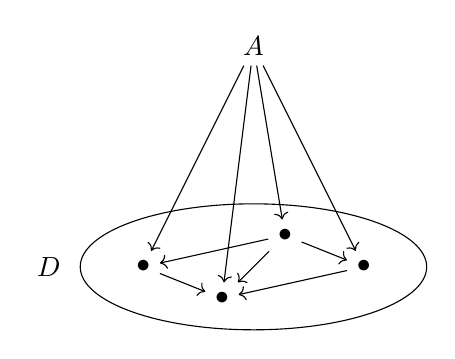
\begin{tikzpicture}[scale=2, link/.style={red,double=black,line width=1.8pt,double distance=0.8pt}]
          \node (A) at (0,0.4) {$A$};
          \node (D1) at (0.2,-0.8) {$\bullet$};
          \node (D2) at (-0.7,-1) {$\bullet$};
          \node (D3) at (0.7,-1) {$\bullet$};
          \node (D4) at (-0.2,-1.2) {$\bullet$};
          \draw [->] (A) -- (D2);
          \draw [->] (A) -- (D3);
          \draw [->] (A) -- (D4);
          \draw [->] (D1) -- (D2);
          \draw [->] (D2) -- (D4);
          \draw [->] (D1) -- (D3);
          \draw [->] (D3) -- (D4);
          \draw [->] (D1) -- (D4);
          \draw [->] (A) -- (D1);
          \draw (0,-1) circle [x radius=1.1cm, y radius=0.4cm];
          \node at (-1.3, -1) {$D$};
        \end{tikzpicture}
      \end{center}
      % picture
      Given cones $(A, (\lambda_j)_{j \in \ob J})$ and $(B, (\mu_j)_{j \in \ob J})$, a morphism of cones between them is a morphism $A \overset{f}\to B$ such that
      \begin{equation*}
        \begin{tikzcd}[column sep=small]
          A \arrow[rr, "f"] \arrow[dr, "\lambda_j"'] && B \arrow[dl, "\mu_j"] \\
                                                    & D(j)
        \end{tikzcd}
      \end{equation*}
      commutes for all $j$.

      We write $\mathbf{Cone}(D)$ for the category of cones over $D$.
    \item \index{limit}\hypertarget{def:limit} A \textbf{limit} for $D$ is a terminal object of $\mathbf{Cone}(D)$, if this exists.
      Dually, we have the notion of cone under a diagram, and of colimit (initial cone under $D$).
  \end{enumerate}
\end{ndef}

Alternatively if $\mathscr{C}$ is \hyperlink{def:lsmall}{locally small} and $J$ is small, we have a functor $\mathscr{C}^{op} \to \mathbf{Set}$ sending $A$ to the set of cones with apex $A$.
A \hyperlink{def:limit}{limit} for $D$ is a representation of this functor.
If $\Delta A$ denotes the constant diagram of shape $J$ with all vertices $A$ and all edges $1_A$, then a cone over $D$ with apex $A$ is the same thing as a natural transformation $\Delta A \to D$.

$\Delta$ is a functor $\mathscr{C} \to [J, \mathscr{C}]$, and $\mathbf{Cone}(D)$ is the category $(\Delta \downarrow D)$ (a \hyperlink{def:comma}{comma category}, reversed).
So to say that every diagram of shape $J$ in $\mathscr{C}$ has a limit is equivalent to saying that $\Delta$ has a \hyperlink{def:adj}{right adjoint}.
(We say $\mathscr{C}$ \textbf{has limits}) of shape $J$.
Dually, $\mathscr{C}$ has colimits of shape $J$ iff $\Delta: \mathscr{C} \to [J, \mathscr{C}]$ has a left adjoint.
\begin{nexample}\leavevmode
  \begin{enumerate}[label=(\alph*)]\label{eg:4.2}
    \item Suppose $J = \emptyset$. There's a unique diagram of shape $J$ in $\mathscr{C}$; a \hyperlink{def:cone}{cone} over it is just an object, and a morphism of cones is a morphism of $\mathscr{C}$.
      So a limit for this empty diagram is a terminal object of $\mathscr{C}$.
      (Dually, a colimit for it is an initial object).
  \end{enumerate}
\end{nexample}
\printindex
\end{document}
